\def\xxactivite{Cours}

\def\xxauteur{Emilien Durif -- Xavier Pessoles}
\fichefalse \proftrue \tdfalse \courstrue

\def\xxnumchapitre{Chapitre 9 \vspace{.2cm}}

\def\xxchapitre{Piles et files}

\def\xxcompetences{%
\textsl{%
\textbf{Savoirs et compétences :}\\
\begin{itemize}[label=\ding{112},font=\color{bleuxp}] 
\item Piles et files.
\end{itemize}
}}

\def\xxfigures{
%
\includegraphics[width=\linewidth]{fractale}
%\\
%\textit{Modèle du pilote hydraulique avec pilotage interactif.}
}%figues de la page de garde


\input{\repRel/Style/pagegarde_cours_minitoc}
\setlength{\columnseprule}{.1pt}

\vspace{2cm}
\pagestyle{fancy}
\thispagestyle{plain}

%Thème : Tris.
% 
%Commentaires :
%\begin{itemize}
%\item algorithmique quadratique : tri par insertion, par sélection;
%\item tri par partition-fusion;
%\item tri par comptage.
%\end{itemize}
%\textit{On fait observer différentes caractéristiques (par exemple2 stable ou non, en place ou non, comparatif ou non ...).}
%





\section{Pile}
\subsection{Présentation}
\begin{defi}{Pile}
Une pile est une structure de données dans laquelle le dernier élément stocké est le premier à en sortir. On parle de principe \textit{LIFO} pour \textit{Last In First Out}. Le dernier élément stocké est appelé \textbf{sommet}.
\end{defi}

Pour gérer une pile, indépendamment de la façon dont elle est implémentée, on suppose exister les opérations élémentaires suivantes : 
\begin{itemize}
\item \texttt{cree\_pile()} qui crée une pile vide;
\item \texttt{empile(p,x)} qui empile l'élément \texttt{x} au sommet de la pile \texttt{p};
\item \texttt{depile(p)} qui supprime le sommet de la pile \texttt{p} et renvoie sa valeur;
\item \texttt{est\_vide(p)} qui teste si la pile \texttt{p}est vide.
\end{itemize}

On peut illustrer la structure de pile par l'image suivante.

\begin{tabular}{p{.3\textwidth}p{.3\textwidth}p{.3\textwidth}}

\centerline{
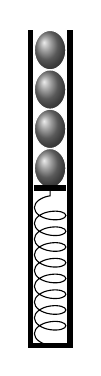
\begin{tikzpicture} [scale=.5]
%\draw[style=help lines] (0, 0) grid (10, 10);
\begin{scope}
\def\n{4};
\foreach \y in {\n,...,7}{ % Une erreur ici que je ne comprends pas
  \draw[yshift=5mm,color=white,ball color=gray,smooth] (0 cm, \y cm) ellipse (.4 cm and .5 cm);
};
\draw[decorate, decoration={coil, segment length = 2 mm, amplitude = 2 mm}] (0, 0) -- (0, \n);
\draw[line width=2pt] (-.5, 8) -- (-.5, 0) -- (.5, 0) -- (.5, 8);
\draw[line width=2pt] (-.4, \n) -- (.4, \n);
\end{scope}
\end{tikzpicture}
}
&

\centerline{
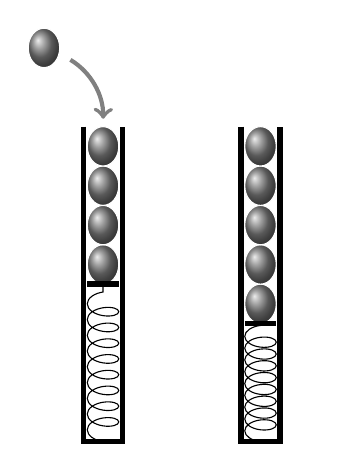
\begin{tikzpicture} [scale=.5]
%\draw[style=help lines] (0, 0) grid (10, 10);
\draw[yshift=5mm,color=white,ball color=gray,smooth] (-1.5 cm, 9.5 cm) ellipse (.4 cm and .5 cm);
% en blanc, juste pour le centrage
\draw[yshift=5mm,color=white] (5.5 cm, 9.5 cm) ellipse (.4 cm and .5 cm);
\draw[->,shorten >=1mm,shorten <=1mm,line width=1.5pt, color=gray] (-1, 9.8) to[bend left] (0, 8);
\begin{scope}
\def\n{4};
\foreach \y in {\n,...,7}{ % Une erreur ici que je ne comprends pas
  \draw[yshift=5mm,color=white,ball color=gray,smooth] (0 cm, \y cm) ellipse (.4 cm and .5 cm);
};
\draw[decorate, decoration={coil, segment length = 2 mm, amplitude = 2 mm}] (0, 0) -- (0, \n);
\draw[line width=2pt] (-.5, 8) -- (-.5, 0) -- (.5, 0) -- (.5, 8);
\draw[line width=2pt] (-.4, \n) -- (.4, \n);
\end{scope}
\begin{scope}[xshift = 40mm]
\def\n{3};
\foreach \y in {\n,...,7}{ 
  \draw[yshift=5mm,color=white,ball color=gray,smooth] (0 cm, \y cm) ellipse (.4 cm and .5 cm);
};
\draw[decorate, decoration={coil, segment length = 1.5 mm, amplitude = 2 mm}] (0, 0) -- (0, \n);
\draw[line width=2pt] (-.5, 8) -- (-.5, 0) -- (.5, 0) -- (.5, 8);
\draw[line width=2pt] (-.4, \n) -- (.4, \n);
\end{scope}
\end{tikzpicture}
}
&

\centerline{
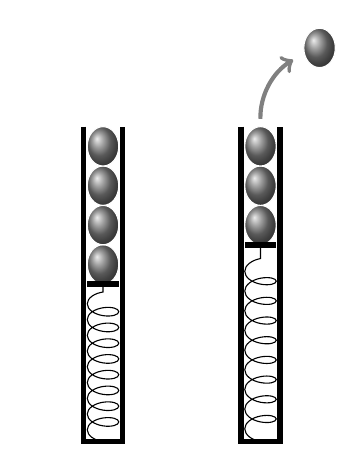
\begin{tikzpicture} [scale=.5]
%\draw[style=help lines] (0, 0) grid (10, 10);
% en blanc, juste pour le centrage
\draw[yshift=5mm,color=white] (-1.5 cm, 9.5 cm) ellipse (.4 cm and .5 cm);
\draw[yshift=5mm,color=white,ball color=gray,smooth] (5.5 cm, 9.5 cm) ellipse (.4 cm and .5 cm);
% \draw[<-,shorten >=1mm,shorten <=1mm,line width=1.5pt, color=gray] (1, 9.8) to[bend right] (0, 8);
\draw[xshift = 40mm,<-,shorten >=1mm,shorten <=1mm,line width=1.5pt, color=gray] (1, 9.8) to[bend right] (0, 8);
\begin{scope}
\def\n{4};
\foreach \y in {\n,...,7}{ % Une erreur ici que je ne comprends pas
  \draw[yshift=5mm,color=white,ball color=gray,smooth] (0 cm, \y cm) ellipse (.4 cm and .5 cm);
};
\draw[decorate, decoration={coil, segment length = 2 mm, amplitude = 2 mm}] (0, 0) -- (0, \n);
\draw[line width=2pt] (-.5, 8) -- (-.5, 0) -- (.5, 0) -- (.5, 8);
\draw[line width=2pt] (-.4, \n) -- (.4, \n);
\end{scope}
\begin{scope}[xshift = 40mm]
\def\n{5};
\foreach \y in {\n,...,7}{ 
  \draw[yshift=5mm,color=white,ball color=gray,smooth] (0 cm, \y cm) ellipse (.4 cm and .5 cm);
};
\draw[decorate, decoration={coil, segment length = 2.5 mm, amplitude = 2 mm}] (0, 0) -- (0, \n);
\draw[line width=2pt] (-.5, 8) -- (-.5, 0) -- (.5, 0) -- (.5, 8);
\draw[line width=2pt] (-.4, \n) -- (.4, \n);
\end{scope}
\end{tikzpicture}
}

\\
\centerline{pile (\textit{stack})}
&
\centerline{empile (\textit{push})}
&
\centerline{dépile (\textit{pop})}\\

\end{tabular}


Théoriquement, chacune de ces opérations doit se faire à \textbf{temps constant} (complexité notée $\mathcal{O}(1)$).
Une des possiblités pour implémenter les piles est d'utiliser le module \texttt{deque}. Chacun des éléments de la pile peut être un objet de type différent.

\begin{lstlisting} 
from collections import deque

# Création d'une pile vide
pile = deque() 

# Test si une pile est vide
len(pile) == 0

# Ajout de l'élément Truc au sommet de la pile
pile.append("Truc")

# Suppression (et renvoi) du sommet d'une pile non vide
sommet = pile.pop()
\end{lstlisting}

\subsection{Applications directes}

\begin{exemple}
\begin{enumerate}
\item \textit{En utilisant le module \texttt{deque} et uniquement les 4 opérations précédemment définies, donner l'implémentation de la fonction \texttt{copy\_pile(p: pile) -> pile}, permettant de faire une copie de la pile.}
\item {Donner la complexité de cette fonction.}
\end{enumerate}

\ifprof
\begin{lstlisting}
from collections import deque

pile = deque()
for i in range(10):
    pile.append(i)


def copy_pile(pile):
    pile_tmp = deque()
    pile_copy = deque()
    
    while pile : 
        pile_tmp.append(pile.pop())
        
    while pile_tmp : 
        el= pile_tmp.pop()
        pile.append(el)
        pile_copy.append(el)
    return pile_copy
\end{lstlisting}
\else
\vspace{5cm}
\fi

\end{exemple}





\begin{exemple}
\begin{enumerate}
\item \textit{En utilisant le module \texttt{deque} et uniquement les 4 opérations précédemment définies, donner l'implémentation de la fonction \texttt{hauteur(p: pile) -> int} renvoyant la hauteur de la pile. Attention, la pile initiale ne doit pas être perdue.}

\item \textit{En utilisant le module \texttt{deque} et uniquement les 4 opérations précédemment définies, donner l'implémentation de la fonction récursive \texttt{hauteur\_rec(p: pile) -> int} renvoyant la hauteur de la pile. La pile initiale peut être perdue, l'utilisateur de la fonction pourra avoir fait  une copie préalable.}

\item \textit{Donner la complexité de cette fonction.}
\end{enumerate}
\ifprof
\begin{lstlisting}
def hauteur(pile) -> int : 
    pile_temp = deque()
    h = 0
    while pile : 
        pile_temp.append(pile.pop())
        h = h+1
    while pile_temp : 
        pile.append(pile_temp.pop())
    return h
    
def hauteur_rec(pile):
    if not pile : 
        return 0
    else :
        pile.pop()
        return 1+hauteur_rec(pile)
\end{lstlisting}
\else
\vspace{10cm}
\fi

\end{exemple}



\begin{exemple}
\textit{En utilisant le module \texttt{deque} et uniquement les 4 opérations précédemment définies, donner l'implémentation de la procédure \texttt{reverse(p: pile) -> None}, procédure pour laquelle les éléments de la pile sont inversés. Donner la complexité de cette fonction.}

\begin{lstlisting}
def reverse(pile):
    pile_tmp = deque()
    pile_tmp2 = deque()

    while pile : 
        pile_tmp.append(pile.pop())
    while pile_tmp : 
        pile_tmp2.append(pile_tmp.pop())
    while pile_tmp2 : 
        pile.append(pile_tmp2.pop())
\end{lstlisting}

\end{exemple}


\section{File}
\subsection{Présentation}
\begin{defi}{File}
Une file est une structure de données dans laquelle le premier élément stocké est le premier à en sortir. On parle de principe \textit{FIFO} pour \textit{First In First Out}. 
\end{defi}

Pour gérer une file, indépendamment de la façon dont elle est implémentée, on suppose exister les opérations élémentaires suivantes : 
\begin{itemize}
\item création d'une file vide;
\item test si une file est vide;
\item rajout d'un élément dans la file;
\item suppression (et renvoi) du premier élément innséré dans la file.
\end{itemize}

Théoriquement, chacune de ces opérations doit se faire à \textbf{temps constant}.

Une des possiblités pour implémenter les files est d'utiliser le module \texttt{deque}. Chacun des éléments de la file peut être un objet de type différent. Dans cette vision des files, les éléments sont ajoutés <<~à droite~>> et sortent de la file <<~par la gauche~>>.

\begin{lstlisting} 
from collections import deque

# Création d'une file vide
file = deque() 

# Teste si une pile est vide
len(file) == 0

# Ajoute l'élément Truc dans la file 
file.append("Truc")

# Suppression (et renvoi) du premier élément inséré dans la file
sommet = pile.popleft()

\end{lstlisting}


\subsection{Applications directes}

\begin{exemple}
\begin{enumerate}
\item \textit{En utilisant le module \texttt{deque} et uniquement les 4 opérations précédemment définies, donner l'implémentation de la fonction \texttt{copy\_file(f: file) -> file}, permettant de faire une copie de la file.}
\item {Donner la complexité de cette fonction.}
\end{enumerate}

\ifprof
\begin{lstlisting}
def copy_file(file):
    file_tmp = deque()
    file_copy = deque()
    while file : 
        file_tmp.append(file.popleft())
        
    while file_tmp : 
        el= file_tmp.popleft()
        file.append(el)
        file_copy.append(el)
    return file_copy
\end{lstlisting}
\else
\vspace{5cm}
\fi

\end{exemple}





\begin{exemple}
\begin{enumerate}
\item \textit{En utilisant le module \texttt{deque} et uniquement les 4 opérations précédemment définies, donner l'implémentation de la fonction \texttt{longueur(f: file) -> int} renvoyant la longueur de la file. Attention, la file initiale ne doit pas être perdue.}

\item \textit{Donner la complexité de cette fonction.}
\end{enumerate}
\ifprof
\begin{lstlisting}
def longueur(file) -> int : 
    file_tmp = deque()
    l = 0
    while file : 
        file_tmp.append(file.popleft())
        l = l+1
    while file_tmp : 
        file.append(file_tmp.popleft())
    return l
\end{lstlisting}
\else
\vspace{5cm}
\fi

\end{exemple}



\begin{exemple}
\textit{En utilisant le module \texttt{deque} et uniquement les 4 opérations précédemment définies, donner l'implémentation de la procédure \texttt{reverse(f: file) -> None}, procédure pour laquelle les éléments de la file sont inversés. Donner la complexité de cette fonction.}
\end{exemple}
